\documentclass[a4paper,12pt]{report}

\usepackage[francais]{babel}
\usepackage[T1]{fontenc}
\usepackage[latin1,utf8]{inputenc}
\usepackage{soul}
\usepackage{lmodern}
\usepackage{amsmath}
\usepackage{amssymb}
\usepackage{mathrsfs}
\usepackage{amsmath}
\usepackage{amsfonts}
\usepackage{amssymb}
\usepackage{graphics}
\usepackage{pgf,tikz}
\usepackage{multirow}
\usepackage{listings}
\usepackage{algorithm}
\usepackage{algorithmic}
\usepackage{graphicx}

\setlength{\parindent}{0cm}
\setlength{\parskip}{1ex plus 0.5ex minus 0.2ex}
\newcommand{\hsp}{\hspace{20pt}}
\newcommand{\HRule}{\rule{\linewidth}{0.5mm}}

\begin{document}

\begin{titlepage}
  \begin{sffamily}
  \begin{center}

    \textsc{ Université Pierre et Marie Curie \\[1cm] \huge Résolution de problèmes}\\[6cm]

    \textsc{\huge \bfseries Résolution de Mots Croisés par un CSP.}\\

    % Title
    \HRule \\[0.4cm]

~~\\
~~\\
    % Author and supervisor
    \begin{minipage}{0.4\textwidth}
      \begin{center} \large
        Renaud \textsc{ADEQUIN}\\
        Nadjet \textsc{BOURDACHE}\\
      \end{center}
    \end{minipage}

    \vfill

    % Bottom of the page
    {\large 04/04/2016}

  \end{center}
  \end{sffamily}
\end{titlepage}

\section*{1. Modélisation par un CSP et résolution}
\begin{enumerate}
\item Pour résoudre ce problème, on propose une modélisation qui consiste à associer une variable à chaque mot de la grille. Les mots de la grille étants numérotés dans l'odre de leurs apparition dans la grille (d'abord les mots horizontaux puis les verticaux). On définit ensuite un ensemble de contraintes pour vérifier la cohérence de la grille générée.

~~\\
\textbf{Variables:}


Pour \textit{m} mots, on a \textit{m} variables : \textit{$Mot_i$} , $\forall$ $i$  $\in$ $\{1, ... , m \}$.

~~\\
\textbf{Domaine:}


Chaque mot de la grille doit appartenir au dictionnaire considéré, notons le $Dict$.
\begin{center}
D(\textit{$Mot_i$}) $=$ $\{ X \in$ $Dict$  : $|X|$ = $|Mot_i|$ $\}$, $\forall$  $i$ $\in$ $\{1, ... , m \}$ .
\end{center}

~~\\
\textbf{Contraintes:}\\
\begin{itemize}
\item Pour toute paire de mots \textit{Mot$_i$} et \textit{Mot$_j$} qui se croisent aux positions \textit{p} pour \textit{Mot$_i$} et \textit{q} pour \textit{Mot$_j$}, on définit la contrainte:
$$\textit{Mot}_i [p]\ =\  \textit{Mot}_j [q] .$$ 

\item Pour modéliser le fait qu'un même mot ne peut apparaître plus d'une fois dans la grille, il suffit d'ajouter la contrainte:
$$ \textit{AllDiff}\ (\textit{Mot}_1, \textit{Mot}_2, \cdots , \textit{Mot}_m)  $$\\
\end{itemize}

\item D'un point de vue algorithmique, nous avons mis en œuvre une classe "Grille". Chaque objet de cette classe représente une instance de mots croisés, et contient une taille, un dictionnaire, une liste de tous les mots de la grille ayant une taille supérieure à 1 ainsi qu'une liste de cases noires.\\
On pourra à partir d'un objet de cette classe, initialiser une grille à partir d'un fichier texte contenant une grille ou en générer une aléatoirement et la sauvegarder dans un fichier après résolution.\\

Nous proposons une interface graphique qui permet d'ouvrir une grille vide ou partielement rempli ou d'en générer une en indiquant sa taille et le poucentage de cases noirs. Nous pouvons aussi à tout moment sauvegarder la grille non/partielement/completement résolue. \\

\item Nous avons développé les algorithmes AC3 et Forward Checking tel qu'ils ont été définis en cours. \\

\ul{Heuristique}:

Nous avons développé plusieurs heuristiques:\\
 - Domaine minimum : qui donne la variable avec le plus petit domaine.\\
 - Max contraintes instance : nous renvoi le mot avec le plus de contraintes avec les variables déjà instanciés.\\
 - Max contraintes : renvoi la viariable avec le plus de contraintes.\\
 
Afin de déterminer l'heuristique la plus appropriée pour les différents algorithmes, nous avons compté le nombre de mots testés pour chaque heuristique.
Après plusieurs tests, nous avons déterminé que la meilleure heuristique pour le Forward Checking était l'heuristique "domaine min". 

Cependant il aurais été plus judicieux de combiner les heuristiques en cas d'égalité, mais le sujet nous indiquait de prendre un choix aléatoire pour plus de diversité.\\

\item En revanche, pour le Conflict BackJumping, afin d'améliorer la résolution, nous avons:
\begin{itemize}
\item Effectué une arc-consistance sur les mots de la grille pour réduire les domaines avant de lancer l'algorithme.
\item Ajouté un Check Forward avant l'appel récursif, ce qui nous permet d'éviter des appels inutiles et d'améliorer encore le temps de résolution des grilles les plus grandes.\\
\end{itemize}

\ul{Heuristique}:

Pour le CBJ, l'heuristique la plus efficace est la même que pour le FC, à savoir "domaine min".\\

\item \ul{Structure}:\\Afin d'améliorer les trois algorithmes, nous avons utilisé une structure d'arbre pour sauvegarder et manipuler les dictionnaires et les domaines des différentes variables.\\
 Cette structure permet un parcours rapide du dictionnaire pour l'initialisation des domaines, et surtout, elle permet accélérer les algorithmes de filtrage, puisqu'elle peut permettre d'éliminer plusieurs mots d'un domaine en supprimant des sous arbres de ce dernier, nous évitant ainsi de devoir parcourir et tester chaque mot du domaine.\\
\end{enumerate}

\section*{2. Expérimentations}


Nous avons effectuer des expérimentations sur les algorithmes programmés, en les appliquant à différentes instances, pour chacune d'entre elles, nous avons calculé une moyennes du temps d'exécution.\\
Pour chaque grille, nous réalisons une courbe qui montre l'évolution du temps de calcul en fonction de la taille des dictionnaires (une moyenne sur un ensemble d'exécution). Nous représentons également par des points les valeurs obtenues pour chaque exécution.\\
Pour chaque test, nous avons limité le temps de calcul à 5min.

\begin{enumerate}


\item Pour le filtrage par AC3, les résultats obtenus pour les différentes grilles sont représentés sur les graphiques ci-dessous.

On voit clairement que le temps du filtrage augmente exponentiellement avec la taille des dictionnaires utilisés. Ce qui se justifie par une plus grande taille du domaines des variables, et donc par plus de valeurs pour lesquels on vérifiera la consistance.

On remarque surtout, que plus la grille contient de mots, plus les temps croissent rapidement lorsqu'on augmente la taille des dictionnaires. Ceci est du au fait qu'il y ai plus de variables, et donc plus de contraintes à vérifier et plus de domaines qui croissent lorsque la taille augmente.\\

\begin{table*}[!h]
\begin{center}
\begin{tabular}{|c|}

\hline
  Grille A\\
\hline   
   \\
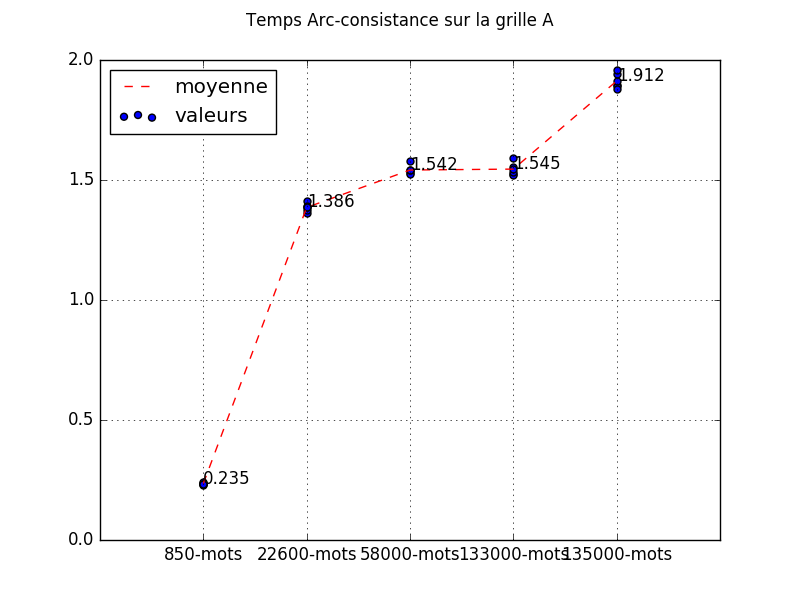
\includegraphics[width=10cm]{AC3_A.png}  \\
\hline

\end{tabular}
\end{center}
\end{table*}

\begin{table*}[!h]
\begin{center}
\begin{tabular}{|c|}
\hline
Grille B \\
\hline 
\\
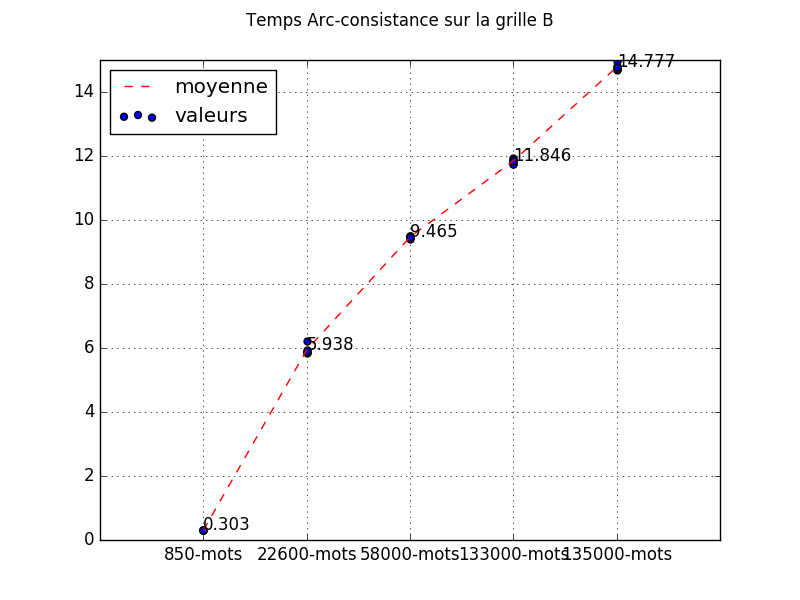
\includegraphics[width=10cm]{AC3_B.png} \\
\hline

\end{tabular}
\end{center}
\end{table*}


\begin{table*}[!h]
\begin{center}
\begin{tabular}{|c|}
\hline
Grille C\\
\hline
  \\
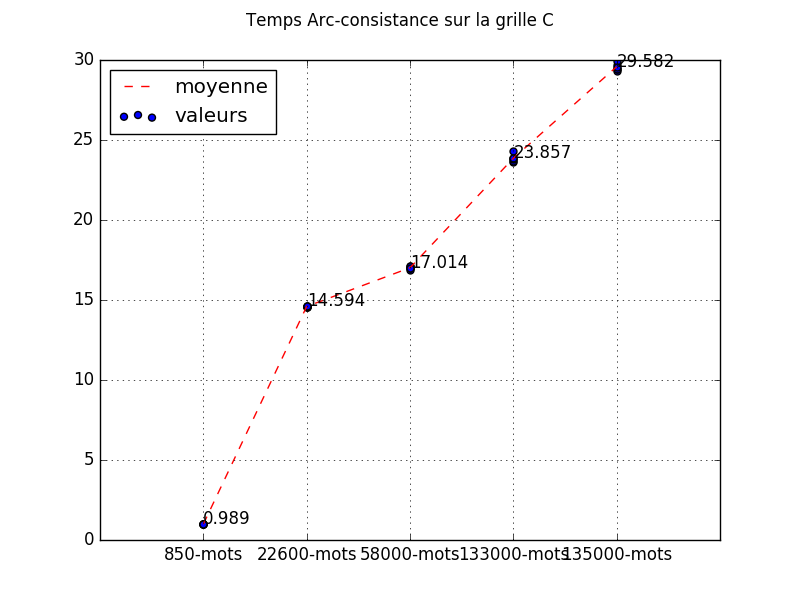
\includegraphics[width=10cm]{AC3_C.png} \\
\hline

\end{tabular}
\end{center}
\end{table*}

\newpage
~~\\
~~\\
~~\\
\item Pour les algorithmes de résolution FC et CBJ, nous avons comparé les résultats des deux algorithmes avec et sans filtrage et avec différentes tailles de grilles et de dictionnaires.\\
Les résultats obtenus sont représenté sur les graphiques suivants.\\

On remarque que le temps de calcul ne dépend pas forcément de la taille des dictionnaires. Pour une même grille, on peut obtenir des changement non monotone du temps de calcul lorsqu'on change la taille des dictionnaires.\\

On remarque aussi que lorsqu'il n'y a pas de solution, comme c'est le cas pour les trois grille avec le dictionnaire de 850 mots, le FC est en général plus rapide que le CBJ.\\

- Plus particulièrement, pour la grille A, on remarque que le filtrage par AC3 préalable n'est bénéfique que pour les petits dictionnaires. Pour les plus grands dictionnaires, la résolution sans filtrage par AC3 demande un temps de calcul beaucoup plus court que lorsqu'on en effectue un. C'est du au grand nombre mots à tester dans les domaines des différentes variables, le temps passé sur le filtrage est donc long et n'est pas compensé par le temps gagné à la résolution.\\

En ce qui concerne l'efficacité des deux algorithmes pour cette grille, aucun des deux n'est nettement meilleur que l'autre, le CBJ (avec ou sans AC3) est plus rapide que le FC (avec ou sans AC3) pour le dictionnaire de 58000 mots mais plus lent pour les dictionnaire de 22600 et 135000 mots. En revanche pour le dictionnaire de 850 mots, les deux algorithmes sont plus ou moins équivalents.


\begin{table*}[!h]
\begin{center}
\begin{tabular}{|c|}

\hline
  Grille A\\
\hline   
   \\
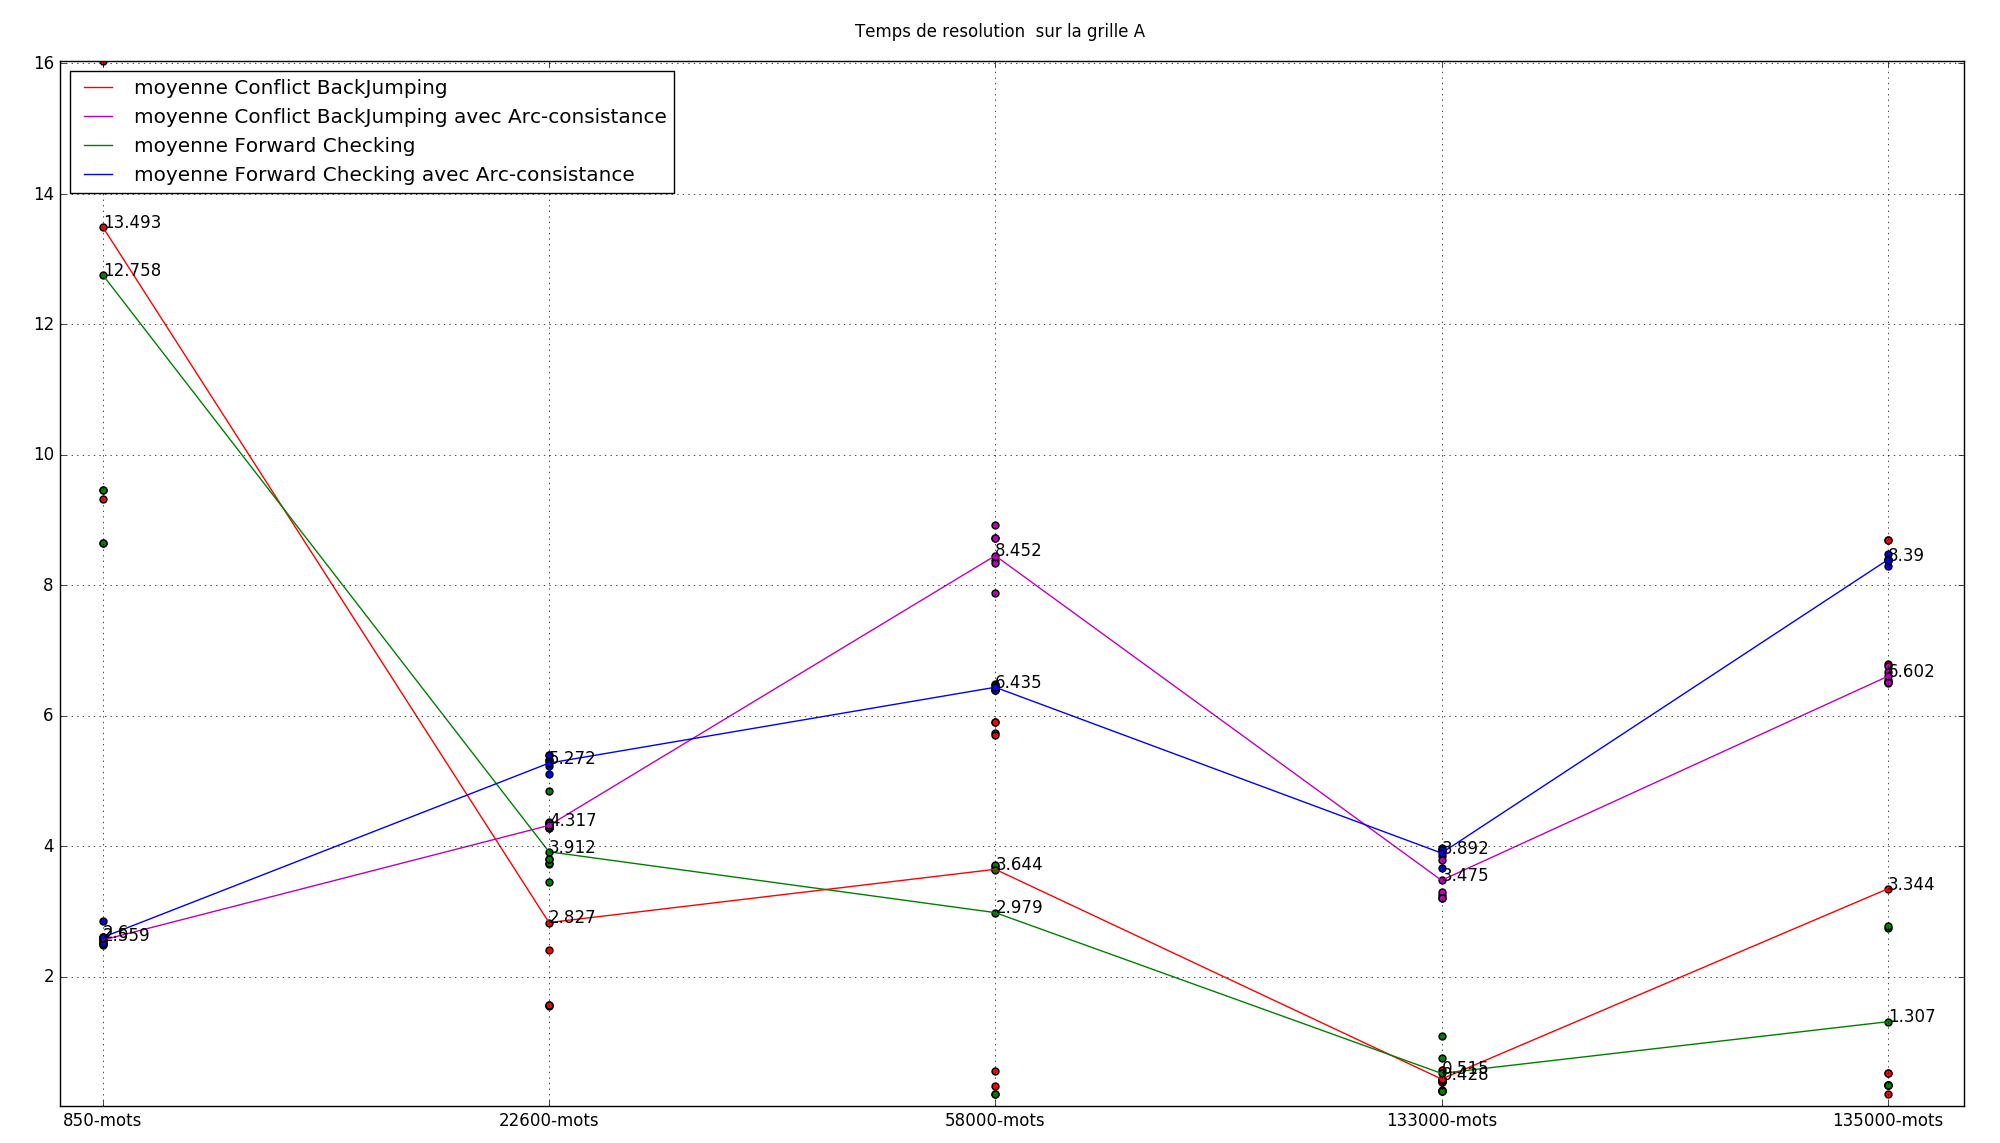
\includegraphics[width=9cm]{Grille_A.png}  \\
\hline


\end{tabular}
\end{center}
\end{table*}

- De même pour la grille B, le filtrage n'accélère le temps de calcul que pour les dictionnaire de petite taille. Même si la différences de temps avec et sans est moins importante que pour la grille A.\\

Pour cette grille, les meilleurs temps ont été obtenus avec le FC. D'ailleurs, sur cette grille, le temps de calcul du FC sur cette grille ne semble pas croitre exponentiellement avec la taille du dictionnaire.\\

\begin{table*}[!h]
\begin{center}
\begin{tabular}{|c|}

\hline
Grille B \\
\hline 
\\
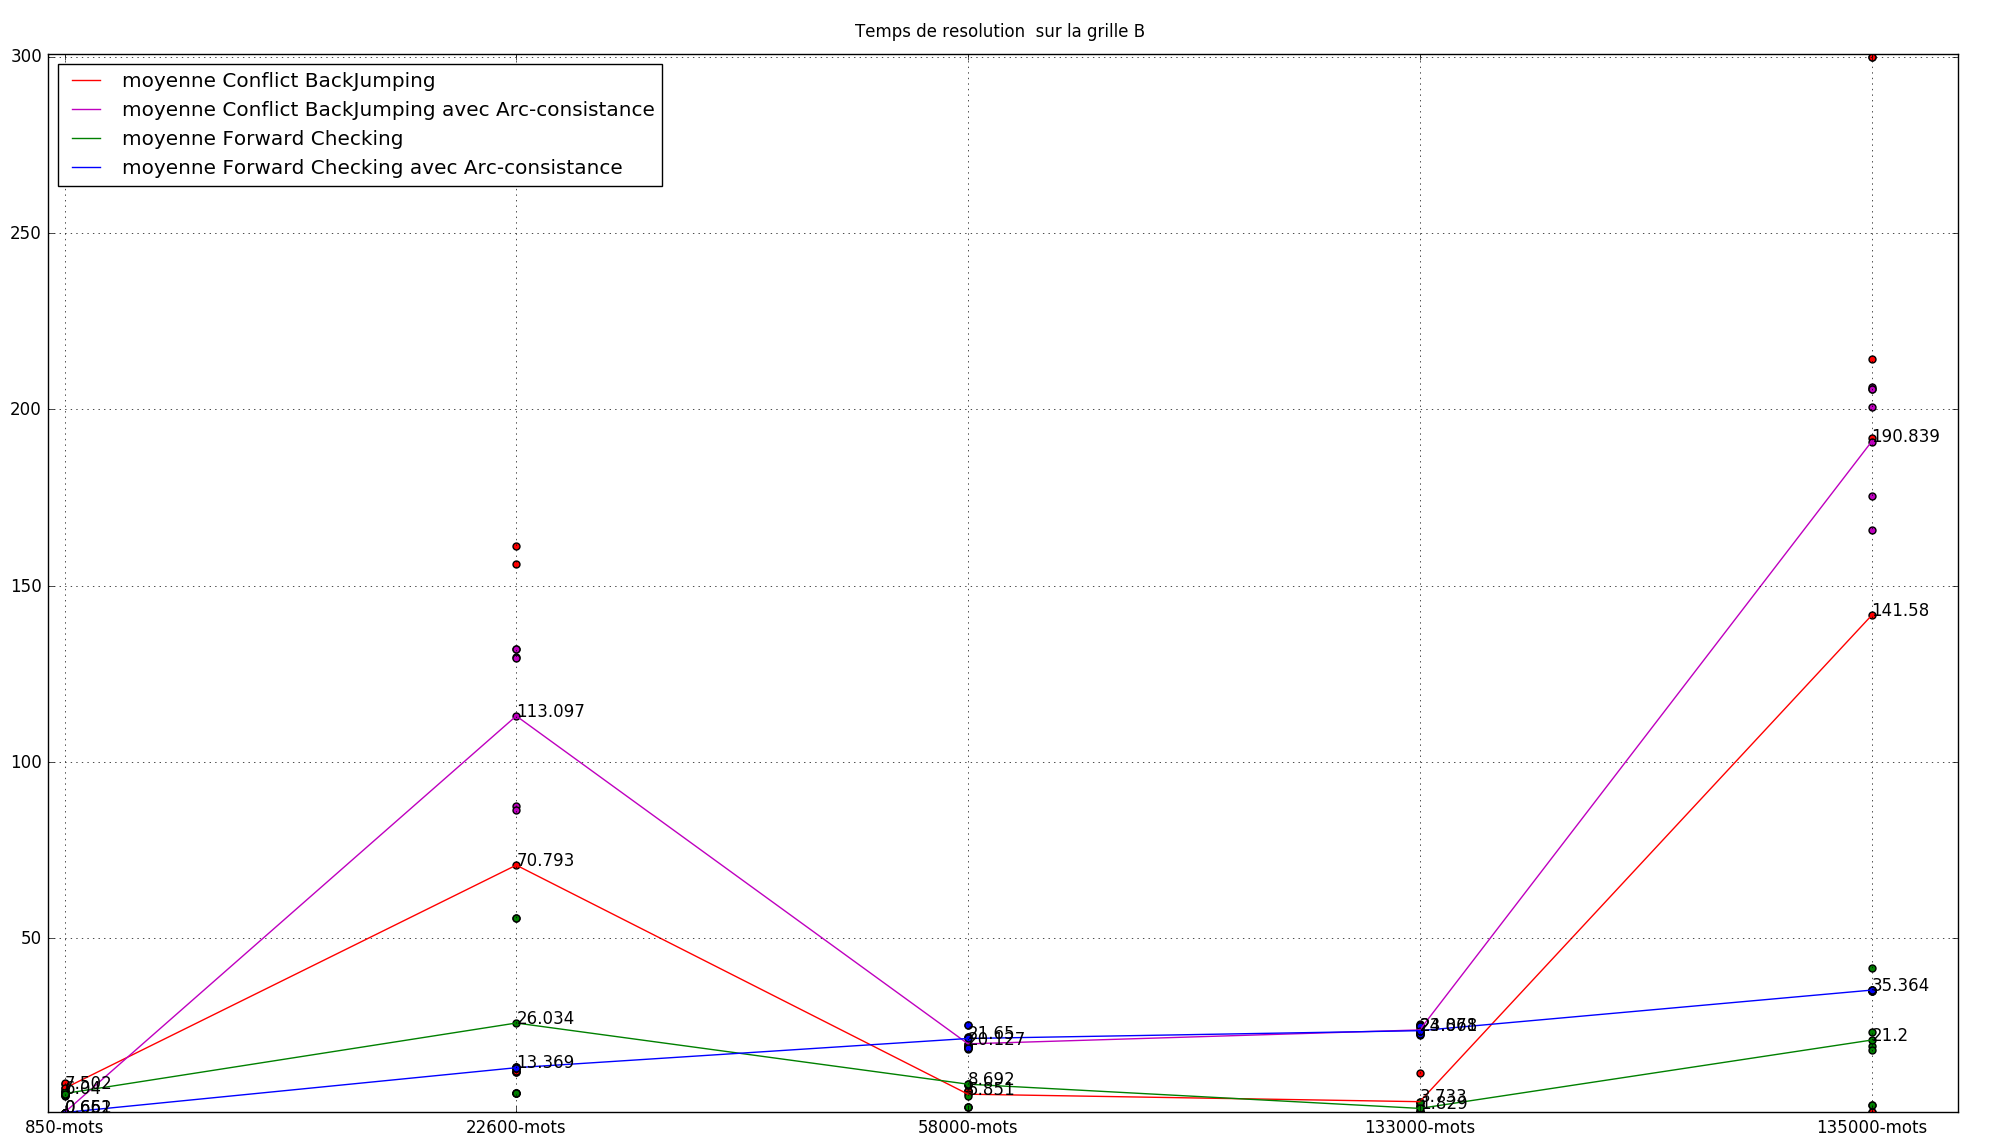
\includegraphics[width=9cm]{Grille_B.png} \\
\hline


\end{tabular}
\end{center}
\end{table*}
\newpage
- En ce qui concerne l'apport du filtrage, on constate les mêmes résultats sur la grille C, le filtrage est plus ou moins bénéfique selon la taille des dictionnaires. \\

On peut remarquer qu'en moyenne, le CBJ (avec ou sans AC3 préalable) est plus rapide que le FC.\\

\begin{table*}[!h]
\begin{center}
\begin{tabular}{|c|}

\hline
Grille C \\
\hline
\\
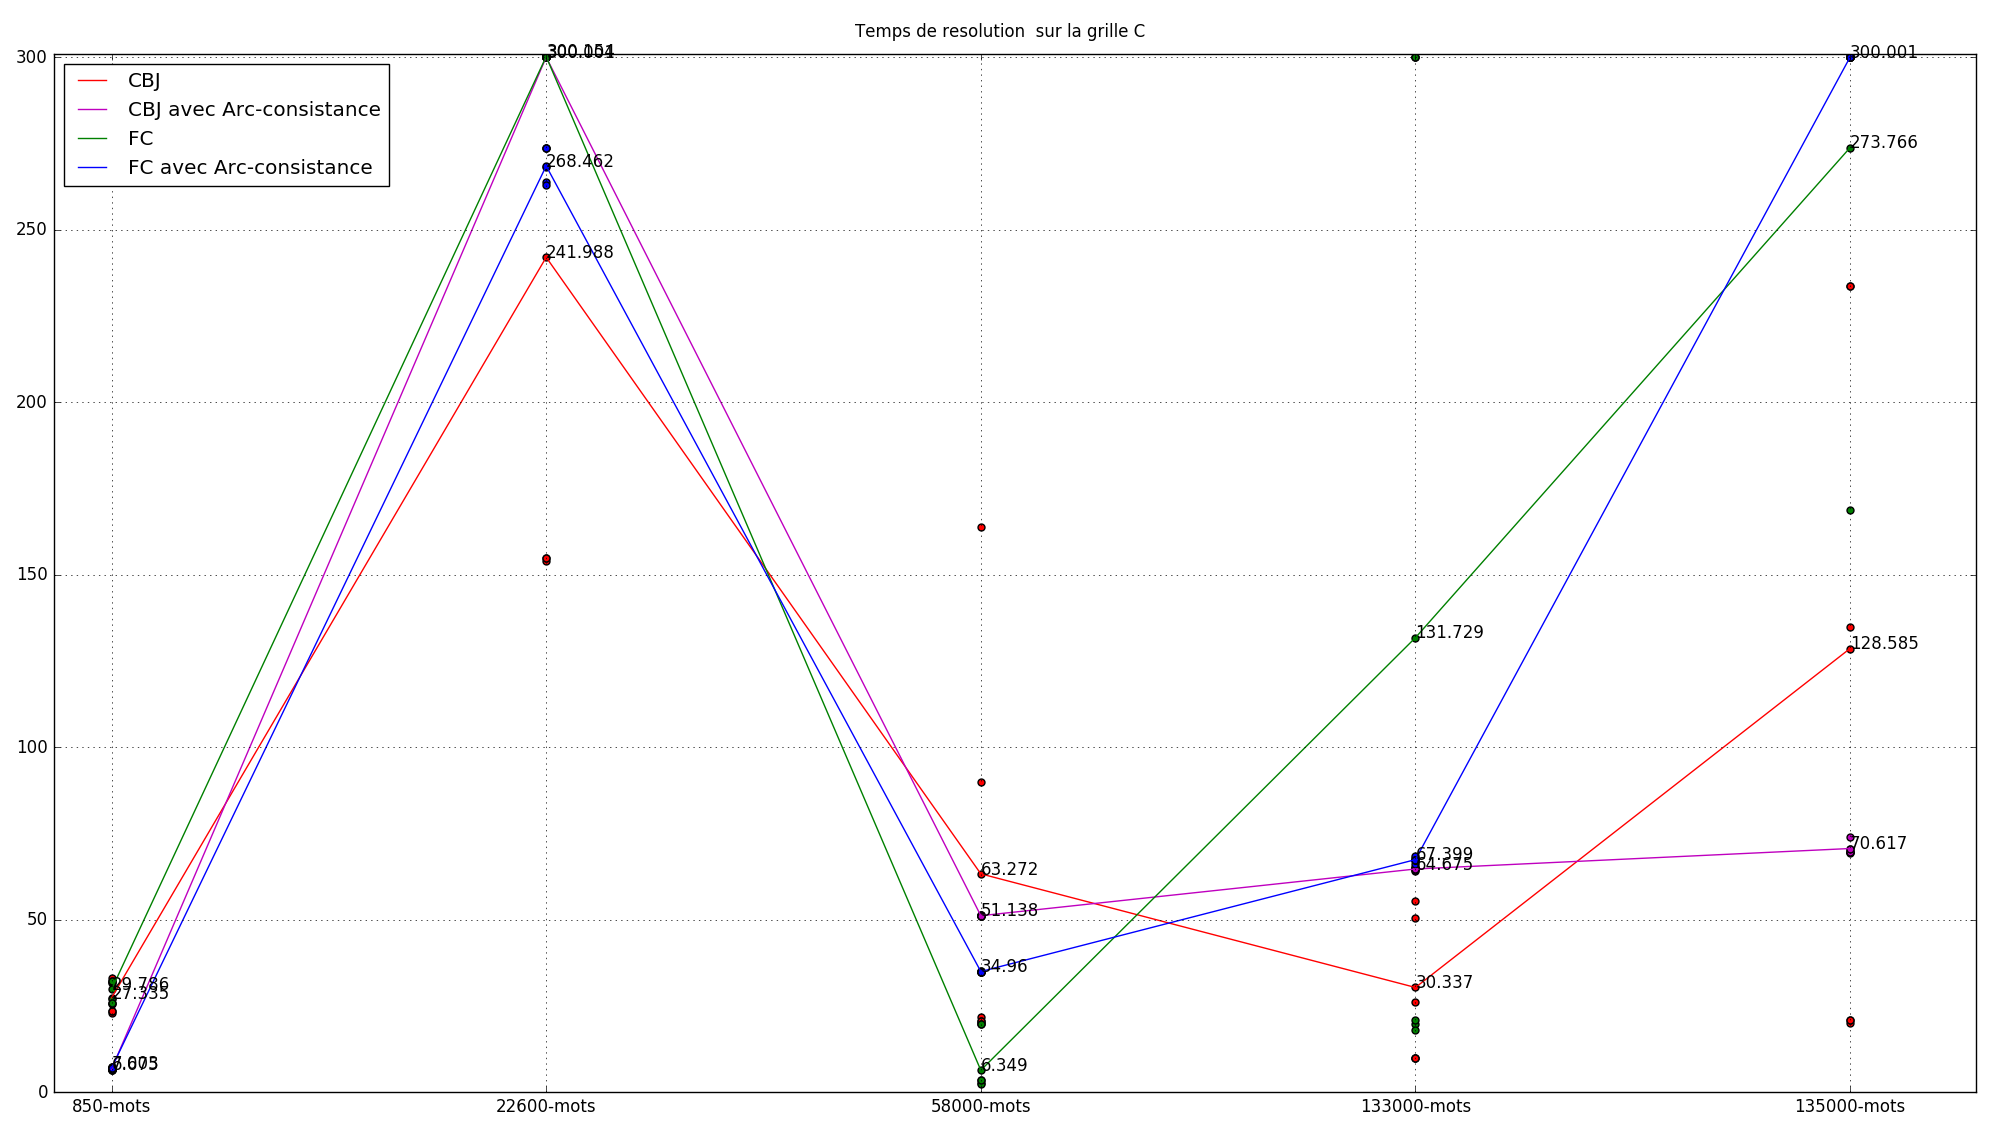
\includegraphics[width=10cm]{Grille_C.png}\\

\hline

\end{tabular}
\end{center}
\end{table*}

\item Pour prolonger les expérimentation, nous avons testé une grille aléatoire de taille 12x12. Nous avons choisi de lui appliquer le CBJ avec AC3 préalable car c'est l'algorithme qui a donné les temps de calcul les plus court pour les grandes tailles de grilles et de dictionnaires.\\

Pour ces tests, nous obtenons des temps assez bons, mis à part pour le dictionnaire de taille 58000 ou on atteint notre "time out" de 5min.

\begin{table*}[!h]
\begin{center}
\begin{tabular}{|c|}

\hline
Grille aléatoire de taille 12x12 \\
\hline
\\
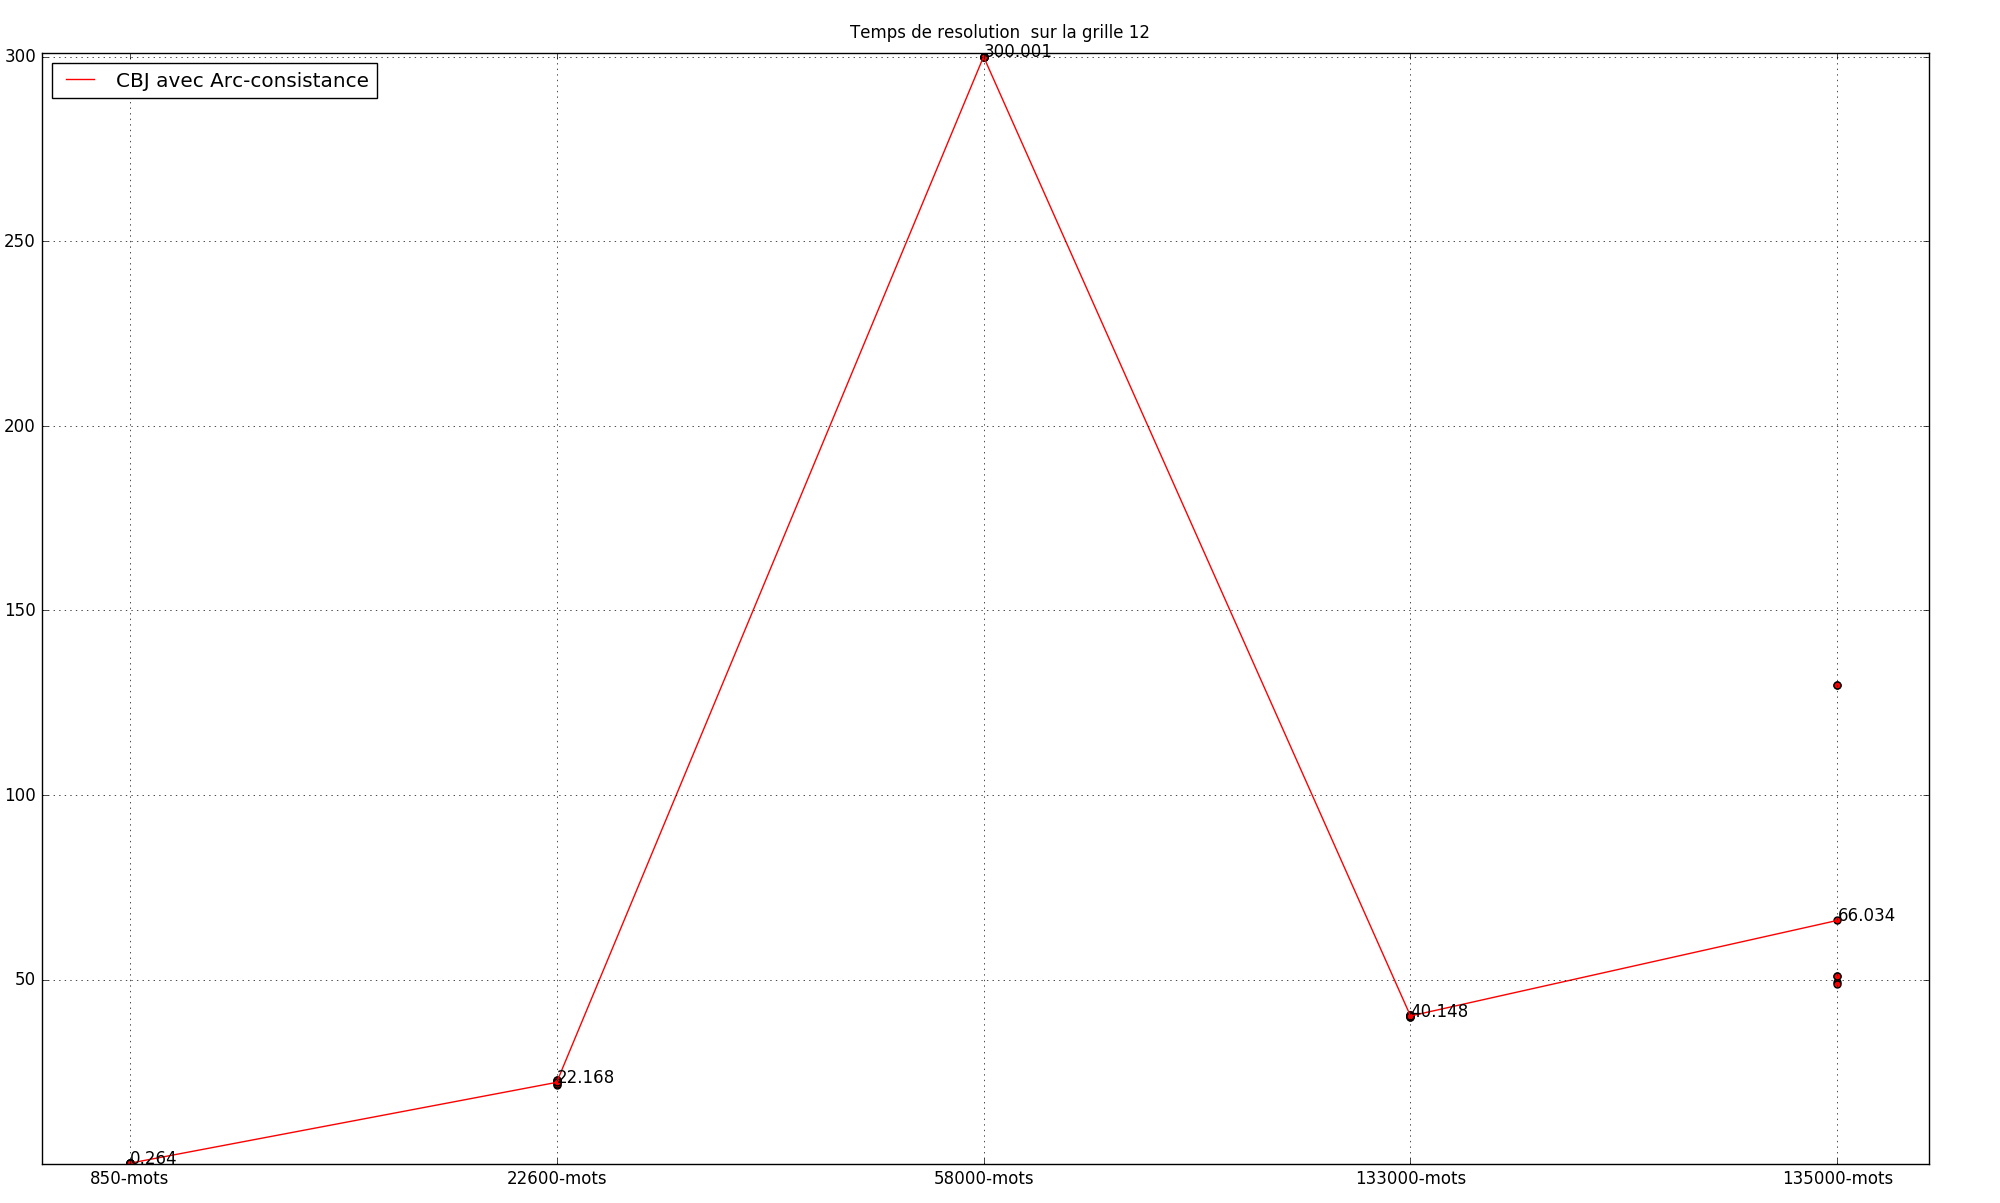
\includegraphics[width=10cm]{12.png}\\

\hline

\end{tabular}
\end{center}
\end{table*}

\end{enumerate}

\section*{3. Extension au cas valué}

\begin{enumerate}

\item Pour modéliser le problème de CSP valué, il suffit de reprendre la modélisation de la question 1.1 en ajoutant des valeurs aux mots du dictionnaire.\\

\ul{Structures de valuations}: 

Pour le Branch \& Bound, on peut proposer la structure de valuation suivante: la valeur d'un nœuds est le minimum entre sa propre valeur (dans le dictionnaire) et celle de son père. La valeur d'une solution est donc la valeur minimum de tous les mots de l'instanciation qui la constitue.\\
L'intérêt de cette valuation est qu'en développant, à chaque itération, le nœud de valeur maximum parmi toutes les feuilles de l'arbre, on peut garantir l'obtention de l'instanciation de valeur maximum sans avoir à parcourir la totalité de l'arbre de recherche.\\
Cette valuation est monotone, car lorsqu'on ajoute un mots à l'instanciation courante, la valeur de la solution courante peut soit diminuer soit stagner, mais ne peut jamais augmenter.\\

\item Nous avons choisi de modéliser le Branch \& Bound sous forme d'une liste de nœuds triés selon leurs valeurs croissantes. Cette liste contiendra uniquement les nœuds susceptibles d'être développé, c'est à dire les feuilles de l'arbre.  \\

A chaque étape, le nœud à développer sera le nœud de valeur maximum, à savoir, le nœud qui se trouve à la dernière position de la liste. En cas d'égalité de valeur, nous choisissons de prendre le nœud le plus profond dans l'arbre.\\
Afin de grader notre liste triée avec une faible complexité, nous effectuons des insertions triées en utilisant deux classes de python, à savoir collections.deque et bisect, qui nous permettent de faire des insertions triées en O(log N).\\

\item Expérimentation: \\
Pour tester l'efficacité de notre Branch \& Bound, nous l'avons appliqué à la grille du TD3, avec des dictionnaires de différentes taille allants de 200 à 700 mots, où les mots en rapport avec le master ANDROIDE ont une valeur de 1 et les autres mots ont une valeur aléatoire comprise entre 0 et 1 exclu.\\
Nous avons obtenu des temps de calcul assez rapide, mais qui augmente exponentiellement à partir de 600 mots.\\
Le graphique suivants montre les résultats obtenus:


\begin{table*}[!h]
\begin{center}
\begin{tabular}{|c|}

\hline
Grille du TD3 \\
\hline
\\
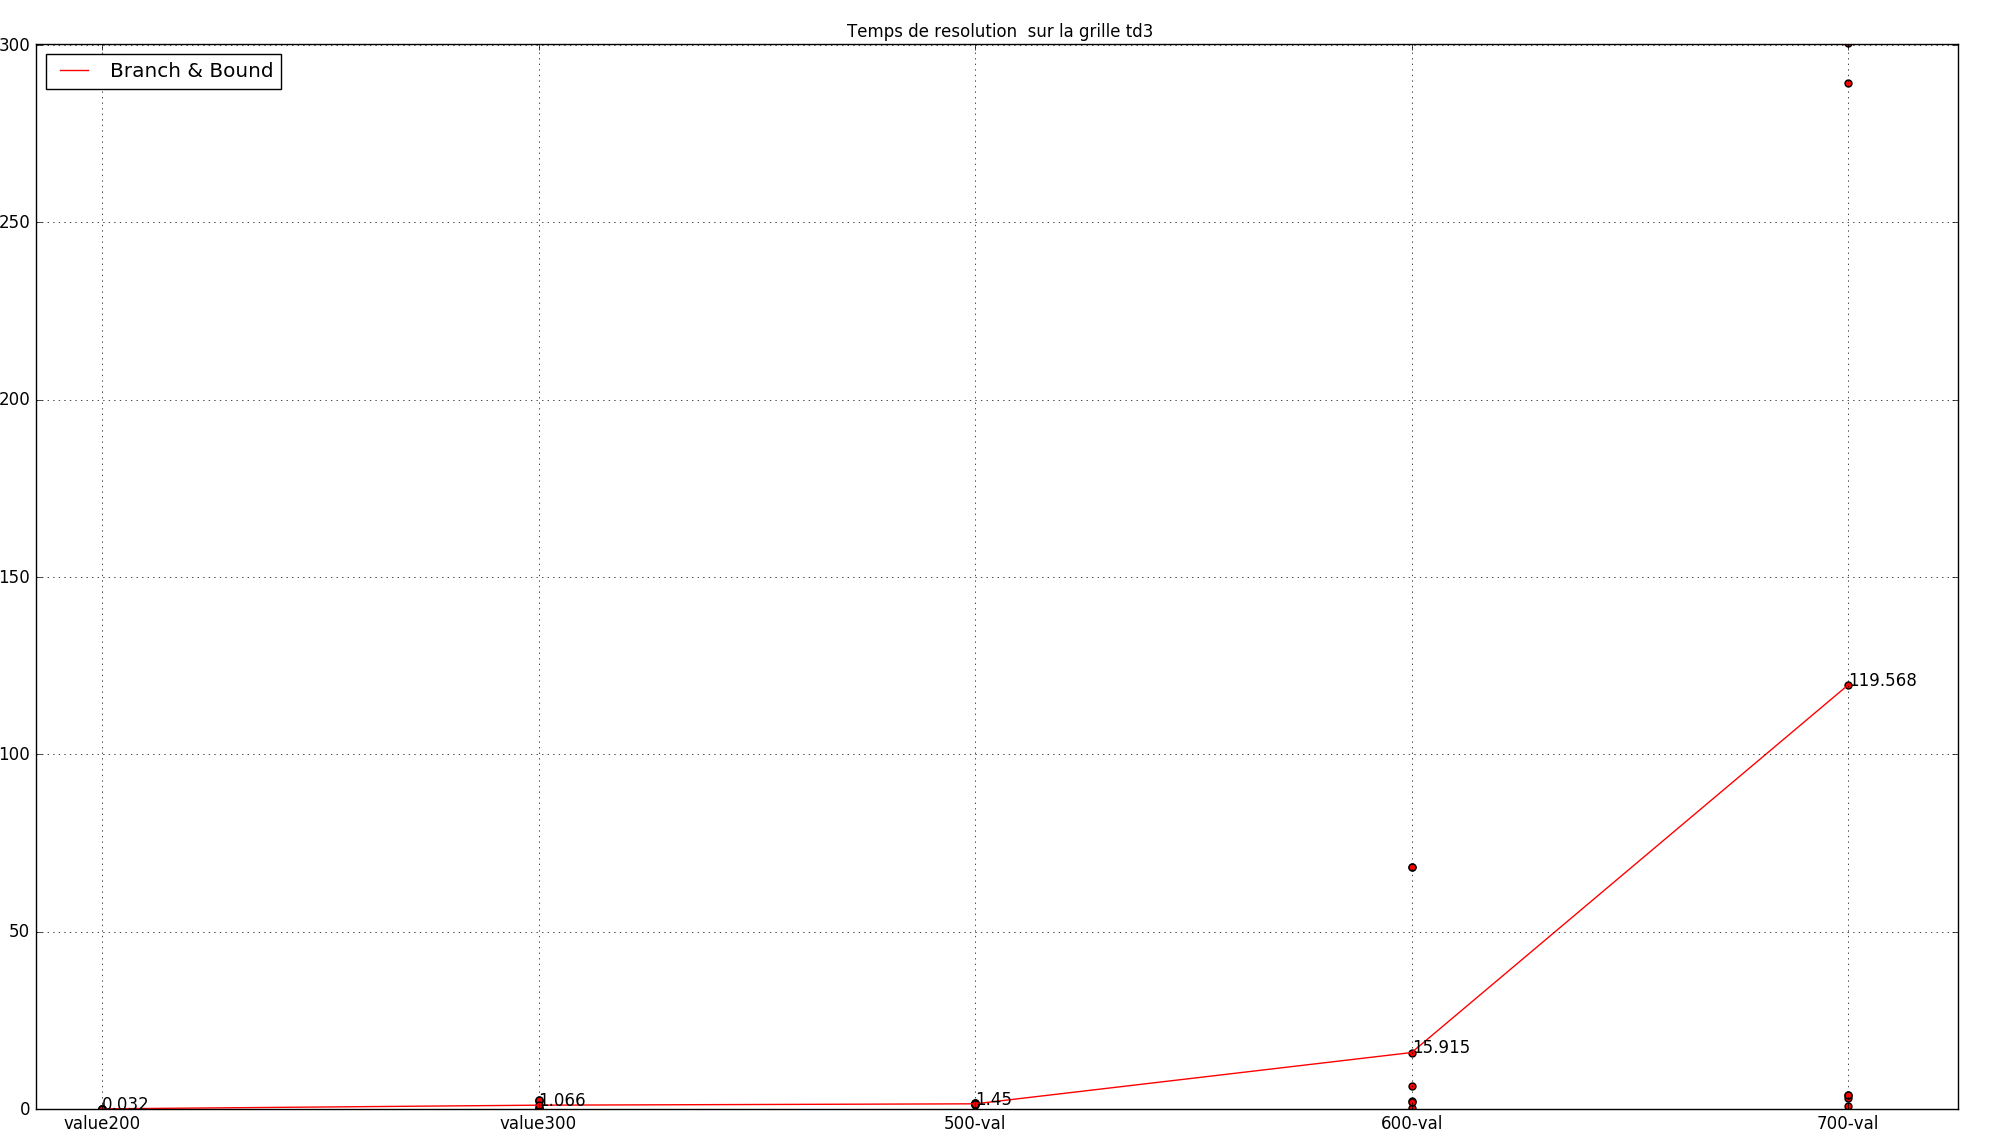
\includegraphics[width=10cm]{BB.png}\\

\hline

\end{tabular}
\end{center}
\end{table*}

\item \textit{Question bonus:} Pour cette question, nous avons mis au point un programme qui crée un dictionnaire contenant les mots d'un texte, et qui associe à chaque mot de taille supérieure à deux sa fréquence d'apparition dans le texte. Pour les mots de taille deux, on associe une valeur aléatoire comprise entre 0 et 1 exclu.\\

\end{enumerate}

\section*{Conclusion}
En conclusion, les algorithmes programmés sont relativement efficaces, mais d'une efficacité non constantes. Cela dépend certainement des heuristiques qui n'ont pas la même efficacité d'une instance à l'autre, de l'ordre dans lequel les mots sont pris dans les dictionnaires mais aussi de l'existence ou non de solutions pour l'instance étudiée.

\end{document}
